\clearpage
\phantomsection

\setcounter{chapter}{3}
\chapter[{MÔ PHỎNG VÀ KIỂM THỬ}]{mô phỏng và kiểm thử}
Để đánh giá độ chính xác của thiết kế, một bước quan trong trong quá trình thiết kế là cần có các bài mô phỏng và các trường hợp kiểm thử. Chương 4 sẽ mô tả chi tiết về một số phương pháp kiểm thử được sử dụng, các điều kiện để đánh giá độ chính xác của kiểm thử, mô hình giúp tự động hóa quá trình kiểm thử.
\section{Cơ sở lý thuyết kiểm thử}
\subsubsection{Lý thuyết về độ bao phủ}
Độ bao phủ (coverage) là phương pháp thống kê trong quá trình kiểm tra thiết kế để xác định được chất lương của quá trình kiểm tra. Độ bao phủ là một yếu tố quan trọng để khẳng định được thiết kế có được kiểm tra theo các yêu cầu đưa ra hay chưa. Từ đó, có thể xem xét tạo ra các bài kiểm tra để đảm bảo bao quát được các trường hợp.

Có hai yếu tố bao phủ thường được đánh giá là độ bảo phủ về mã nguồn (code coverage) và độ bao phủ về mặt chức năng (functional coverage). Trong đó, độ bao phủ về mã nguồn sẽ đánh giá xem là các điều kiện ví dụ các điều kiện rẽ nhánh có được thực hiện ít nhất 1 lần hay không, do đó nó không có ý nghĩa về mặt đánh giá độ chính xác của thiết kế mà chỉ đảm bảo rằng bộ kiểm thử sinh ra đã bao quá được hết mã nguồn. Độ bao phủ về mặt chức năng sẽ đánh giá độ bao phủ của thiết kế dựa trên tính năng đã được kiểm tra. Do đó, việc định nghĩa ra các tính năng nào cần được đánh giá sẽ quyết định chất lượng của độ bao phủ về mặt chức năng. Độ bao phủ về mặt mã nguồn thường được thu thập từ các phần mềm sử dụng để thiết kế ví dụ Vivado, QuetaSim,... Trong khi đó, độ bao phủ về mặt chức năng phải do kỹ sư tự định nghĩa, kỹ sư cần tự định nghĩa điểm cần bao phủ. Ví dụ về kiểm tra về mặt chức năng, giả sử kỹ sư cần kiểm tra một biến có thay đổi theo như mong muốn hay không. Nếu đúng, biến đấy phải thay đổi giá trị từ 3 -> 5 -> 7 chẳng hạn. Độ bao phủ về mặt mã nguồn chỉ biết là biến đấy đã thành 3, 5 hoặc 7 mà không thể đánh giá được về mặt thứ tự xuất hiện.

\subsubsection{Các phương pháp kiểm thử}
Trong thiết kế nói chung, sau khi đã thiết kế được các mạch từ mã nguồn hoặc thông qua các công cụ, kỹ sư cần thiết kế các bài kiểm thử để đánh giá tính đúng đắn của thiết kế. Thông thường, đối với thiết kế số, kỹ sư sẽ thiết kế ra các phương pháp kiểm thử trực tiếp (directed testing). Khi sử dụng phương pháp này, kỹ sư sẽ nhìn vào các yêu cầu kỹ thuật, viết ra các trường hợp có thể xảy ra và kiểm tra nó với một kết quả đã biết trước. Để kiểm tra, kỹ sư có thể nhìn dạng sóng mô phỏng, sử dụng các điều kiện để kiểm tra. Đây là một phương pháp nhanh, phù hợp với kỹ sư cần kiểm tra ngay lập tức thiết kế là đúng hay sai, nhưng sẽ khó để đảm bảo hoàn toàn về mặt thiết kế. Giả sử, nếu thiết kế có 10, 100 tín hiệu đầu vào, vậy nếu viết tay và tính toán các trường hợp kiểm thử sẽ rất tốn thời gian và có thể dễ mắc đến các sai lầm.

Vậy để có thể kiểm tra được toàn bộ thiết kế một cách đầy đủ, các kỹ sư sẽ thiết kế ra các kích thích sinh ngẫu nhiên với ràng buộc (constrained-random stimulus). Các kích thích này sẽ sinh ra các tín hiệu ngẫu nhiên giá trị, tuy nhiên phải tuân theo các ràng buộc cho trước. Ví dụ, kỹ sư có thể yêu cầu khi sinh ra dữ liệu điểm ảnh, thì tín hiệu hợp lệ phải ở mức 1. Từ đó, kỹ sư có thể kiểm tra được nhiều trường hợp hơn với những dữ liệu ngẫu nhiên đó. Hình \ref{fig:verificationEva} mô tả biểu đồ phân tích thời gian và độ bao phủ của các bộ kiểm thử. Có thể thấy, với cách tạo ra các kích thích trực tiếp, thời gian để đạt độ bao phủ cần thiết là rất lớn, trong khi đó với các kích thích được sinh ngẫu nhiên với các ràng buộc, thời gian này đã giảm đi một cách đáng kể.

\begin{figure}[!ht]
\centering
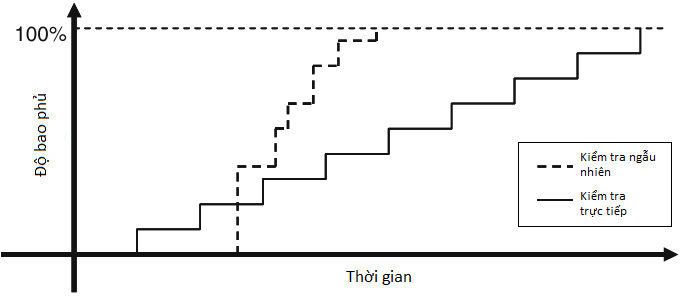
\includegraphics[width=\linewidth]{figures/verificationEva.png}
\caption{Biểu đồ phân tích thời gian và độ bao phủ của các bộ kiểm thử}
\label{fig:verificationEva}
\end{figure}

\section{Phương pháp xây dựng kiểm thử}
Hình \ref{fig;testComponents} mô tả các thành phần cơ bản của một bộ kiểm tra, bao gồm testbench sẽ sinh ra các kích thích đầu vào và sau đó thu thập các dữ liệu đầu ra.
Trong khi thiết kế, kỹ sư sẽ cần kiểm tra ngay lập tức chức năng của một hoặc nhiều mô đun để đảm bảo tính chính xác một cách chưa đầy đủ, tức là kiểm tra mô đun đó đã hoạt động đúng tính năng mong muốn hay chưa, tuy nhiên có thể có những trường hợp ngoại lệ mà kỹ sư có thể không nghĩ đến. Do đó, thường thì kỹ sư sẽ kiểm tra bằng cách tạo ra các bộ kiểm thử với kích thích sinh trực tiếp để tiết kiệm về mặt thời gian. Do đó, đối với các mô đun nhỏ, sinh viên sẽ tự đưa ra các bộ kích thích trực tiếp và sau đó kiểm tra kết quả với đầu ra đã có trước. 

\begin{figure}[!ht]
	\centering
	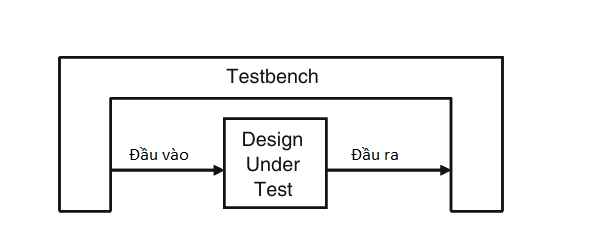
\includegraphics[width=\linewidth]{figures/testComponents.png}
	\caption{Các thành phần cơ bản của một bộ kiểm tra}
	\label{fig:testComponents}
\end{figure}

Tuy nhiên, khi cần kiểm tra tính đúng đắn của toàn bộ thiết kế, sinh viên sẽ sử dụng một thiết kế kiểm tra gọi là kiểm tra lớp (layered test-bench) được viết bằng ngôn ngữ SystemVerilog. Bộ kiểm thử lớp này có vẻ sẽ phức tạp hơn so với thiết kế trực tiếp, tuy nhiên thực tế nó sẽ giúp quản lý các công việc một cách dễ dàng hơn bằng cách chia mã nguồn thành các thành phần nhỏ hơn. Hình \ref{fig:layeredLayer} mô tả các lớp của bộ kiểm tra lớp và hình \ref{fig:layeredTestbench} mô tả các đầy đủ các thành phần của bộ kiểm tra lớp.

\begin{figure}[!ht]
	\centering
	\begin{minipage}[t]{0.48\linewidth}
		\centering
		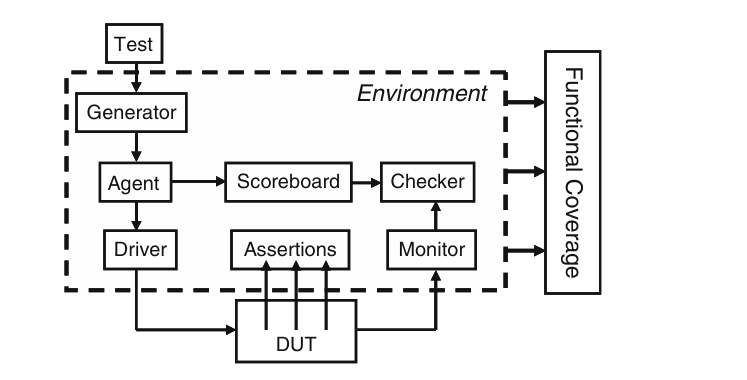
\includegraphics[width=\linewidth]{figures/layeredTestbench.png}
		\caption{Các thành phần của bộ kiểm tra lớp}
		\label{fig:layeredTestbench}
	\end{minipage}
	\hfill
	\begin{minipage}[t]{0.48\linewidth}
		\centering
		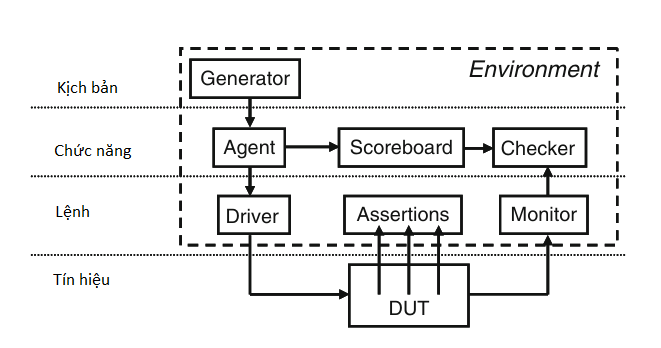
\includegraphics[width=\linewidth]{figures/layeredLayer.png}
		\caption{Các lớp của bộ kiểm tra lớp}
		\label{fig:layeredLayer}
	\end{minipage}
\end{figure}

Ở lớp dưới cùng là lớp tín hiệu, lớp này sẽ bao gồm các tín hiệu được kết nối với testbench. Lớp phía trên ngay nó là lớp lệnh. Các tín hiêu vào của DUT được điều khiển bởi các lệnh. Các dữ liệu đầu ra của DUT sẽ được bộ giám sát thu được và chuyển chúng thành các lệnh. Lớp chức năng sẽ nhận được các phiên từ các lớp cao hơn và chuyển chúng thành các lệnh riêng biệt hoặc các phiên. Các lệnh này cũng sẽ được gửi tới bộ scoreboard để dự đoán kết quả và bộ kiểm tra sẽ ....

\section{Đánh giá kết quả kiểm thử}

